\documentclass[ejs]{imsart}

\RequirePackage{amsthm,amsmath,amsfonts}
\RequirePackage[authoryear]{natbib}
\RequirePackage[colorlinks,citecolor=blue,urlcolor=blue]{hyperref}
\RequirePackage{graphicx}
\RequirePackage{bm, bbm}

% settings
\pubyear{2022}
\volume{0}
\issue{0}
\firstpage{1}
\lastpage{8}
\arxiv{2005.05506}

\startlocaldefs
\numberwithin{equation}{section}
\theoremstyle{plain}
\newtheorem{theorem}{Theorem}[section]
 \newtheorem{proposition}{Proposition}
 \newtheorem{claim}{Claim}
 \newtheorem{lemma}{Lemma}
 \newtheorem{corollary}{Corollary}
 \newtheorem{question}{Question}
 \newtheorem{assumption}{Assumption}
 \theoremstyle{definition}
 \newtheorem{definition}{Definition}
   \newtheorem{setting}{Setting}
 \theoremstyle{remark}
 \newtheorem{remark}{Remark}
 \newtheorem{example}{Example}

\newcommand{\iid}[0]{i.i.d.\xspace}
 \newcommand{\dist}[2]{\mathrm{dist}\!\left({#1},{#2}\right)} % distance
 \newcommand{\one}[1]{{\mathbbm{1}}_{{#1}}}
 \newcommand{\inner}[2]{\langle{#1},{#2}\rangle} % Inner product
 \newcommand{\norm}[1]{\left\lVert{#1}\right\rVert}
 \newcommand{\PP}[1]{\textnormal{Pr}\!\left\{{#1}\right\}} % Probability
 \newcommand{\EE}[1]{\mathbb{E}\left[{#1}\right]} % Expectation
 \newcommand{\Ep}[2]{\mathbb{E}_{#1}\left[{#2}\right]}
 \newcommand{\EEst}[2]{\mathbb{E}\left[{#1}\ \middle| \ {#2}\right]} % Conditional expectation
 \newcommand{\PPst}[2]{\text{Pr}\!\left\{{#1}\ \middle| \ {#2}\right\}} % Conditional probability
 \newcommand{\ee}[1]{\mathbf{e}_{{#1}}}
 \newcommand{\ident}{\mathbf{I}}
 \newcommand{\ones}{\mathbf{1}}
 \newcommand{\zeros}{\mathbf{0}}
 \def\independenT#1#2{\mathrel{\rlap{$#1#2$}\mkern2mu{#1#2}}}
 \newcommand\independent{\protect\mathpalette{\protect\independenT}{\perp}}
 \newcommand{\iidsim}{\stackrel{\mathrm{iid}}{\sim}}
 \newcommand{\indsim}{\stackrel{\independent}{\sim}}
 \newcommand{\notate}[1]{\textcolor{red}{\textbf{[#1]}}}
 \newcommand{\ignore}[1]{}
 \renewcommand{\Pr}[2]{\mathcal{P}_{{#1}}\left({#2}\right)} % projection
 \newcommand{\Prp}[2]{\mathcal{P}_{{#1}}^{\perp}\left({#2}\right)}
 \newcommand{\pr}[1]{\mathcal{P}_{{#1}}}
 \newcommand{\prp}[1]{\mathcal{P}_{{#1}}^{\perp}}
 \newcommand{\eps}{\epsilon}
 \newcommand{\lam}{\lambda}

 \let\emptyset\varnothing
 
 \newcommand{\prx}{\bm X} 
 \newcommand{\prxu}{\underline{\bm X}} 
 \newcommand{\srx}{X}
 \newcommand{\srxu}{\underline X}
 \newcommand{\sfx}{x}
 \newcommand{\pfx}{\bm x}
 
\newcommand{\prz}{\bm Z} 
 \newcommand{\przu}{\underline{\bm Z}} 
\newcommand{\srz}{Z}
\newcommand{\srzu}{\underline Z}
\newcommand{\sfz}{z}
\newcommand{\pfz}{\bm z}
 
 \newcommand{\prxk}{{{\widetilde{\bm X}}}}
 \newcommand{\srxk}{\widetilde X}
 \newcommand{\sfxk}{\widetilde x}
 
 \newcommand{\pry}{{\bm Y}}
 \newcommand{\pfy}{{\bm y}}
 
  \newcommand{\pryu}{\underline{\bm Y}} 
 \newcommand{\sry}{Y}
 \newcommand{\sryu}{\underline Y}
 \newcommand{\sfy}{y}
 
\newcommand{\seps}{\epsilon}
\newcommand{\peps}{\bm \epsilon}
 \newcommand{\sepsu}{\underline \epsilon}
 \newcommand{\pepsu}{\underline{\bm \epsilon}}

\newcommand{\smu}{\mu}
\newcommand{\pmu}{\bm \mu}
\newcommand{\smuu}{\underline \mu}
\newcommand{\pmuu}{\underline{\bm \mu}}

\newcommand{\sSigma}{\Sigma}
\newcommand{\pSigma}{\bm \Sigma}
\newcommand{\sSigmau}{\underline \Sigma}
\newcommand{\pSigmau}{\underline{\bm \Sigma}}

 
 \newcommand{\D}{\mathcal D}
 
\def\CRT{\textnormal{CRT}}

\endlocaldefs

\begin{document}

\begin{frontmatter}
\title{On the power of conditional independence testing under model-X \support{Support information of the article.}}
\runtitle{A Sample Document}

\begin{aug}
\author{\fnms{Eugene} \snm{Katsevich}\thanksref{t1,t2}\ead[label=e1]{ekatsevi@wharton.upenn.edu}}
\and
\author{\fnms{Aaditya} \snm{Ramdas}\thanksref{t3}\ead[label=e2]{aramdas@stat.cmu.edu}}

\address{Department of Statistics and Data Science, University of Pennsylvania\\
Department of Statistics and Data Science, Carnegie Mellon University\\
Machine Learning Department, Carnegie Mellon University \\
\printead{e1,e2}}

\thankstext{t1}{Some comment}
\thankstext{t2}{First supporter of the project}
\thankstext{t3}{Second supporter of the project}
\runauthor{F. Author et al.}

\end{aug}

\begin{abstract}
       For testing conditional independence (CI) of a response $Y$ and a predictor $X$ given covariates $Z$, the model-X (MX) framework has been the subject of active methodological research, especially in the context of MX knockoffs and their application to genome-wide association studies. In this paper, we study the power of MX CI tests, yielding quantitative insights into the role of machine learning and providing evidence in favor of using likelihood-based statistics in practice. Focusing on the conditional randomization test (CRT), we find that its conditional mode of inference allows us to reformulate it as testing a point null hypothesis involving the conditional distribution of $X$. The Neyman-Pearson lemma implies that a likelihood-based statistic yields the most powerful CRT against a point alternative. We obtain a related optimality result for MX knockoffs. Switching to an asymptotic framework with arbitrarily growing covariate dimension, we derive an expression for the power of the CRT against local semiparametric alternatives in terms of the prediction error of the machine learning algorithm on which its test statistic is based. Finally, we exhibit a resampling-free test with uniform asymptotic Type-I error control under the assumption that only the first two moments of $X$ given $Z$ are known.
\end{abstract}

\begin{keyword}[class=MSC]
\kwd[Primary ]{60K35}
\kwd{60K35}
\kwd[; secondary ]{60K35}
\end{keyword}

\begin{keyword}
\kwd{sample}
\kwd{\LaTeXe}
\end{keyword}
\tableofcontents
\end{frontmatter}

\section{Introduction}

\subsection{Conditional independence testing and the MX assumption}

Given a predictor $\prx \in \mathbb R^{d}$, response $\pry \in \mathbb R^{r}$, and covariate vector $\prz \in \mathbb R^{p}$ drawn from a joint distribution $(\prx, \pry, \prz) \sim \mathcal L$, consider testing the hypothesis of conditional independence (CI),
\begin{equation}
H_0: \pry \independent \prx\ |\ \prz \quad \text{versus} \quad H_1: \pry \not \independent \prx\ |\ \prz,
\label{conditional-independence}
\end{equation}
using $n$ data points 
\begin{equation}
\label{eq:xyz}
(\srx, \sry, \srz) \equiv \{(\srx_i, \sry_i, \srz_i)\}_{i = 1, \dots, n} \overset{\text{i.i.d.}}\sim \mathcal L. 
\end{equation}
This fundamental problem---determining whether a predictor is associated with a response after controlling for a set of covariates---is ubiquitous across the natural and social sciences. To keep an example in mind throughout the paper, consider $\pry \in \mathbb R^1$ cholesterol level, $\prx \in \{0,1,2\}^{10}$ the genotypes of an individual at 10 adjacent polymorphic sites, and $\prz \in \{0,1,2\}^{500,000}$ the genotypes of the individual at other polymorphic sites across the genome. Such data $(\srx, \sry, \srz)$ would be collected in a genome-wide association study (GWAS), with the goal of testing for association between the 10 polymorphic sites of interest and cholesterol while controlling for the other polymorphic sites~\eqref{conditional-independence}. CI testing is also connected to causal inference: with appropriate unconfoundedness assumptions, Fisher's sharp null hypothesis of no effect of a (potentially non-binary) treatment $\prx$ on an outcome $\pry$ implies conditional independence. While we do not work in a causal framework, we draw inspiration from connections to causal inference throughout.

As formalized by Shah and Peters \cite{Shah2018}, the problem \eqref{conditional-independence} is fundamentally impossible without assumptions on the distribution $\mathcal L(\prx,\pry, \prz)$, in which case no asymptotically uniformly valid test of this hypothesis can have nontrivial power against \emph{any} alternative. In special cases, the problem is more tractable, for example if $\prz$ has discrete support, or if we were willing to make (semi)parametric assumptions on the form of $\mathcal L(\pry|\prx, \prz)$ (henceforth ``model-$Y|X$''). We will not be making such assumptions in this work. Instead, we follow the lead of Candes et al. \cite{CetL16}, who proposed to avoid assumptions on $\mathcal L(\pry|\prx, \prz)$, but assume that we have access to $\mathcal L(\prx|\prz)$:\footnote{Candes et al. actually require that the full joint distribution $\mathcal L(\prx,\prz)$ is known, but this is because they also test for conditional associations between $\prz$ and $\pry$. We focus only on the relationship between $\prx$ and $\pry$ given $\prz$ and therefore require a weaker assumption.} 
\begin{equation} \label{eq:modelX}
\textit{model-X (MX) assumption}: \mathcal L(\prx| \prz)=  f^*_{\prx|\prz} \text{ for some known } f^*_{\prx|\prz}.\footnote{\textcolor{blue}{We implicitly assume that $\mathcal L$ has a density with respect to some dominating measure on $\mathbb R^{1+1+p}$, and that all conditional densities are well-defined almost surely. Here and throughout the paper, we identify probability distributions with their densities with respect to the appropriate dominating measure.}} 
\end{equation}
Candes et al.\ argue that while both model-$Y|X$ and MX are strong assumptions---especially when $p,d$ are large---in certain cases much more is known about $\prx | \prz$ than about $\pry|\prx, \prz$. In the aforementioned GWAS example, $\prx|\prz$ reflects the joint distribution of genotypes at SNPs across the genome, which is well described by hidden Markov models from population genetics \cite{SetC17}. On the other hand, the distribution $\pry|\prx,\prz$ represents the genetic basis of a complex trait, about which much less is known. In the context of (stratified) randomized experiments, the distribution $\mathcal L(\prx | \prz)$ is the propensity function \cite{Imai2004} (the analog of the propensity score for non-binary treatments \cite{Rosenbaum1983}) and is experimentally controlled. In general causal inference contexts, the MX assumption can be viewed as the assumption that the propensity function is known. 

\subsection{MX methodology and open questions}

Testing CI hypotheses in the MX framework has been the subject of active methodological research. The most popular methodology is MX knockoffs \cite{CetL16}. This method is based on the idea of constructing synthetic negative controls (knockoffs) for each predictor variable in a rigorous way that is based on the MX assumption; see Section~\ref{sec:knockoffs-overview} for a brief overview. Rapid progress has been made on the construction of knockoffs in various cases \cite{SetC17,Romano2019a,Bates2019,Huang2019} and on the application of this methodology to GWAS \cite{SetC17, SetS19}. The conditional randomization test (CRT) \cite{CetL16}, initially less popular than knockoffs due to its computational cost, is receiving renewed attention as computationally efficient variants are proposed, such as the holdout randomization test (HRT) \cite{Tansey2018}, the digital twin test \cite{Bates2020}, and the distilled CRT (dCRT) \cite{Liu2020}. The dCRT in particular is a promising methodology because it combines good power and computational speed; we focus on this variant of the CRT is Sections~\ref{sec:weakening} and~\ref{sec:asymptotic-power} of this paper. We introduce the general CRT methodology next, while deferring the introduction of the dCRT to Section~\ref{sec:weakening}. 

We start with any test statistic $T(\srx, \sry, \srz)$ measuring the association between $\prx$ and $\pry$, given $\prz$. Usually, this statistic involves learning some estimate $\widehat f_{\pry|\prx,\prz}$ based on machine learning, e.g. the magnitude of the fitted coefficient for $\prx$ (when $\text{dim}(\prx) = 1$) in a cross-validated lasso~\cite{T96} of $\sry$ on $\srx$ and $\srz$ \cite{CetL16}. To calculate the distribution of $T$ under the null hypothesis~\eqref{conditional-independence}, first define a matrix  $\srxk \in \mathbb R^{n \times d}$, where the $i$th row $\srxk_i$ is a sample from $\mathcal L(\prx \mid \prz = \srz_i)$. In other words, for each sample $i$, resample $\srx_i$ based on its distribution conditional on the observed covariate values $Z_i$ in that sample. We then use these resamples to build a null distribution $T(\srxk, \sry, \srz)$, from which the upper quantile
\begin{equation}
\color{blue}C(\sry,\srz)\color{black} \equiv Q_{1-\alpha}[T(\srxk, \sry, \srz)|\sry,\srz]
	\label{upper-quantile}
\end{equation}
may be extracted \textcolor{blue}{(the dependence on $\alpha$ left implicit)}, where the randomness is over the resampling distribution $\srxk |  \sry, \srz$. Finally, the CRT rejects if the original test statistic exceeds this quantile:

\begin{equation}
	\label{eq:randomized-CRT}
	\phi^{\CRT}_T(\srx,\sry,\srz) \equiv 
	\begin{cases}
		1, \quad &\text{if }  T(\srx, \sry, \srz) > C(\sry,\srz); \\
		\gamma, \quad &\text{if }  T(\srx, \sry, \srz) = C(\sry,\srz); \\
		0, \quad &\text{if }T(\srx, \sry, \srz) < C(\sry,\srz).
	\end{cases}
\end{equation}
In order to accommodate discreteness, the CRT makes a randomized decision $\gamma$ when $T(\srx, \sry, \srz) = C(\sry,\srz)$ so that the size of the test is exactly $\alpha$. In practice, the threshold $C(\sry,\srz)$ is approximated by computing $T(\srxk^b, \sry, \srz)$ for a large number $B$ of Monte Carlo resamples $\srxk^b \sim \srx|\srz$. For the sake of clarity, this paper considers only the ``infinite-$B$" version of the CRT as defined by~\eqref{upper-quantile} and \eqref{eq:randomized-CRT}. In the causal inference setting, the CRT can be viewed as a variant of Fisher's exact test for randomized experiments that incorporates strata of covariates \cite{Zheng2008,Hennessy2016}, basing inference on rerandomizing the treatment to the units. 

The CI testing problem under MX has benefited from several methodological innovations, but fundamental questions regarding power and optimality have received less attention. Therefore, in this paper we address the following two primary questions:
\begin{enumerate}
	\item[Q1.] Are there ``optimal" test statistics for MX methods, in any sense?
	\item[Q2.] What is the precise connection between the performance of the machine learning algorithm and the power of the resulting MX method?
\end{enumerate}
To the best of our knowledge, Q1 has not been considered before, while Q2 has only been indirectly addressed in the context of lasso-based knockoffs \cite{Weinstein2017, Liu2019, Fan2020, Weinstein2020} and CRT \cite{Wang2020b, Celentano2020}. The present paper complements these existing works by considering arbitrary machine learning methods. We summarize our findings next.

\subsection{Our contributions}

We find that for the MX CI problem, the CRT is more natural to analyze; it is simpler to analyze than MX knockoffs and is applicable for testing even a single conditional independence hypothesis. Thus, we focus mainly on the CRT in the present paper. We obtain the following nontrivial answers to the questions posed above.

\paragraph{A1: Conditional inference leads to finite-sample optimality against point alternatives.}

While the composite nonparametric alternative of the CI problem~\eqref{conditional-independence} suggests that we cannot expect to find a uniformly most powerful test, we may still ask what is the most powerful test against a point alternative. \textcolor{blue}{Restricting our attention to tests valid conditionally on $(\sry, \srz)$ (as the CRT is)} allows us to reduce the composite null to a point null. We can therefore apply the Neyman-Pearson lemma to show (Section~\ref{sec:power}) that the optimal conditionally valid test against a point alternative $\mathcal L$ with $\mathcal L(\pry|\prx,\prz) = \bar f_{\pry|\prx,\prz}$ is the CRT based on the likelihood test statistic:
\begin{equation}
	T^{\text{opt}}(\srx; \sry, \srz) \equiv \prod_{i = 1}^n \bar f(\sry_i|\srx_i, \srz_i).
\end{equation}
The same statistic yields the most powerful one-bit $p$-values for MX knockoffs (Section~\ref{sec:knockoffs}). Despite the simplicity of this result, it has not been derived before and appears central to the design of powerful test statistics. Since the model for $Y|X,Z$ is unknown, this result provides our first theoretical indication of the usefulness of machine learning models to learn this distribution (Q2). A2 below gives a more quantitative answer to Q2.

\paragraph{A2: The prediction error of the machine learning method impacts the asymptotic efficiency of the dCRT but not its consistency.}

It has been widely observed that the better the machine learning method approximates $\pry|\prx,\prz$, the higher power the MX method will have. We put this empirical knowledge on a theoretical foundation by expressing the asymptotic power of the dCRT in terms of the prediction error of the underlying machine learning method (Section~\ref{sec:asymptotic-power}). In particular, we consider semiparametric alternatives of the form
\begin{equation}
	H_1: \mathcal L(\pry|\prx,\prz) = N(\prx^T\beta + g(\prz),\sigma^2).
	\label{parametric-alternative-intro}
\end{equation}
We analyze the power of a dCRT variant that employs a separately trained estimator $\widehat g$ in an asymptotic regime where $d = \text{dim}(\prx)$ remains fixed while $p = \text{dim}(\prz)$ grows arbitrarily with the sample size $n$. We find that this test is consistent no matter what $\widehat g$ is used, while its asymptotic power against local alternatives $\beta_n = h/\sqrt{n}$ depends on the limiting mean-squared prediction error of $\widehat g$ (denoted $\mathcal E^2$) and the limiting expected variance $\mathbb E[\text{Var}[\prx | \prz]]$ (denoted $s^2$). For example, if $d = 1$, the
\begin{equation*}
	\begin{split}
		\text{dCRT power converges to that of normal location test under alternative } N\smash{\left(\frac{hs}{\sqrt{\sigma^2 + \mathcal E^2}},1\right)}.
	\end{split}
\end{equation*}
This represents the first explicit quantification of the impact of machine learning prediction error on the power of an MX method. \\

On the way to addressing Q2, we additionally establish a third result (Section~\ref{sec:weakening}) that may be of independent interest:

\paragraph{A resampling-free second-order approximation to the dCRT is equivalent to the dCRT and controls Type-I error under weaker assumptions.}

It was recently pointed out that if $\mathcal L(\prx|\prz)$ is Gaussian, then the resampling distribution of the dCRT test statistic can be found in closed form without actual resampling \cite{Liu2020}. Here we show that the resampling-free dCRT based on the first two moments of $\mathcal L(\prx|\prz)$ is asymptotically equivalent to the dCRT based on $\mathcal L(\prx|\prz)$ itself. Furthermore, we show the former test has asymptotic Type-I error control under the
\begin{equation}
	\begin{split}
		&\textit{MX(2) assumption:} \text{ the first two moments of $\prx|\prz$ are known, i.e.} \\
		&\mathbb E_{\mathcal L}[\prx|\prz] = \mu(\prz) \text{ and } \text{Var}_{\mathcal L}[\prx|\prz] = \Sigma(\prz) \text{ for known } \mu(\cdot), \Sigma(\cdot).
		\label{MX(2)-intro}
	\end{split}
\end{equation}
This assumption is weaker than the full MX assumption, complementing existing work \cite{Huang2019, Barber2020} on weakening assumptions for MX methods. It also suggests that the resampling-free dCRT may be used in place of the usual dCRT while achieving similar power and controlling Type-I error asymptotically.


\paragraph*{}

These advances shed new light on the nature of the MX problem and can inform methodological design. Our results handle multivariate $\prx$, arbitrarily correlated designs in the model for $\prx$, and any black-box machine learning method to learn $\widehat g$. 
\paragraph{Notation.}

Recalling equations~\eqref{conditional-independence} and \eqref{eq:xyz}, population-level variables (such as $\prx,\pry,\prz$) are denoted in boldface, while samples of these variables (such as $\srx_i,\sry_i,\srz_i$) are denoted in regular font. Note that boldface does \textit{not} distinguish between scalars, vectors, and matrices, as it is sometimes employed. The dimensions of the object in this paper will be clear from context. All vectors are treated as column vectors. 
% For example, $\srx \in \mathbb R^{n \times d}, \sry \in \mathbb R^{n \times r}, \srz \in \mathbb R^{n \times p}$. 
We often use uppercase symbols to denote both random variables and their realizations (for either population- or sample-level quantities), but use lowercase to denote the latter when it is important to make this distinction. We use $\mathcal L$ to denote the joint distribution of $(\prx,\pry,\prz)$, though we sometimes use this symbol to denote the joint distribution of $(\srx,\sry,\srz)$ as well. We use the symbol ``$\equiv$" for definitions. We denote by $c_{d,1-\alpha}$ the $1-\alpha$ quantile of the $\chi^2_d$ distribution, and by $\chi^2_d(\lambda)$ the non-central $\chi^2$ distribution with $d$ degrees of freedom and noncentrality parameter $\lambda$.


\section{The most powerful CRT against point alternatives} \label{sec:power}

In this section, we seek the most powerful CRT against a point alternative. To accomplish this, we make the observation---\textcolor{blue}{implicit in earlier works}---that the CRT is valid not just unconditionally but also conditionally on $\sry, \srz$ (Section~\ref{sec:bridge}). The latter conditioning step reduces the composite null to a point null. This reduction allows us to invoke the Neyman Pearson lemma to find the most powerful test  (Section~\ref{sec:NP}). Proofs are deferred to the appendix.

\subsection{CRT is conditionally valid and implicitly tests a point null} \label{sec:bridge}

Let us first formalize the definition of a level $\alpha$ test of the MX CI problem. The null hypothesis is defined as the set of joint distributions compatible with conditional independence and with the assumed model for $\prx|\prz$:
\begin{equation}
	\label{eq:null-under-modelX}
	\begin{split}
		\mathscr L^{\text{MX}}_0(f^*) &\equiv \mathscr L_0 \cap \mathscr L^{\text{MX}}(f^*) \\
		&\equiv \{\mathcal L: \prx \independent \pry \mid \prz\} \cap \{\mathcal L: \mathcal L(\prx|\prz) = f^*_{\prx|\prz}\}\\
		&= \{\mathcal L: \mathcal L(\prx,\pry,\prz) = f_{\prz} \cdot f^*_{\prx|\prz} \cdot f_{\pry|\prz} \text{ for some } f_{\prz}, f_{\pry|\prz} \}.
	\end{split}
\end{equation}
A test $\phi: (\mathbb R^{d} \times \mathbb R^r \times \mathbb R^p)^n \rightarrow [0,1]$ of the MX CI problem is said to be level $\alpha$ if
\begin{equation}
	\sup_{\mathcal L \in \mathscr L^{\text{MX}}_0(f^*)} \mathbb E_{\mathcal L}[\phi(\srx, \sry, \srz)] \leq \alpha.
	\label{marginal-validity}
\end{equation}
Recall that the CRT critical value $C(\sry, \srz)$ is defined via conditional calibration~\eqref{upper-quantile}. As is known to those familiar with MX, this implies that any CRT $\phi = \phi_T^{\text{CRT}}$ not only has level $\alpha$ in the sense of definition~\eqref{marginal-validity} but also has level $\alpha$ \textit{conditionally} on $\sry$ and $\srz$:
\color{blue}
\begin{equation}
\sup_{\mathcal L \in \mathscr L_0^{\textnormal{MX}}(f^*)}\ \mathbb E_{\mathcal L}[\phi(\srx, \sry, \srz)|\sry, \srz] \leq \alpha \quad \text{almost surely}.
\label{eq:conditional-validity}
\end{equation}
\color{black}

One special property of such conditionally valid tests $\phi$ is that they can be viewed as testing a \textit{point null} rather than the original \textit{composite null} \eqref{conditional-independence}. To see this, we view $\phi \equiv \phi(\srx;\sry,\srz)$ as a \textit{family} of hypothesis tests, indexed by $(\sry, \srz)$, for the distribution $\mathcal L(\srx|\sry,\srz)$. Note that under the MX assumption,
\small
\begin{equation}
\mathcal L \in \mathscr L_0^{\text{MX}}(f^*) \Longrightarrow \mathcal L(\srx = \sfx|\sry = \sfy, \srz = \sfz) = \prod_{i = 1}^n  f^*(\sfx_i | \sfz_i).
\label{point-null}
\end{equation}
\normalsize
In words, fixing $Y,Z$ at their realizations $\sfy,\sfz$ and viewing only $\srx$ as random, $\mathcal L(\srx|\sry = \sfy, \srz = \sfz)$ equals a fixed product distribution for any null $\mathcal L$. This yields a conditional point null hypothesis, with respect to which $\phi^{\CRT}_T(\sfx;\sfy,\sfz)$ is a level-$\alpha$ test for \textcolor{blue}{almost every} $(\sfy, \sfz)$. Note that the observations $\srx_i$ in this conditional distribution are independent \textit{but not identically distributed} due to the different conditioning events in~\eqref{point-null}.

\color{blue}
We emphasize that the aforementioned observations have been under the hood of MX papers, and the existence of a single null distribution from which to resample $\srxk$ is central to the very definition of the CRT. Nevertheless, we find it useful to state explicitly what has thus far been largely left implicit. Indeed, viewing the CRT through the conditional lens~\eqref{eq:conditional-validity} is the starting point that allows us to bring classical theoretical tools to bear on its analysis. We start doing so by considering point alternatives below.
\color{black}

\subsection{The most powerful conditionally valid test} \label{sec:NP}

Viewing the CRT as a test of a point null hypothesis, we can employ the  Neyman-Pearson lemma to find the most powerful CRT (in fact, the most powerful conditionally valid test) against point alternatives. The following theorem states that the likelihood ratio with respect to the (unknown) distribution $\pry|\prx, \prz$ is the most powerful CRT test statistic against a point alternative.

\begin{theorem} \label{prop:crt-optimality}
	Let $\bar{\mathcal L} \in \mathscr L^{\text{MX}}(f^*)$ be an alternative distribution, with $\bar{\mathcal L}(\pry|\prx,\prz) = \bar f_{\pry|\prx,\prz}$. The likelihood of the data $(\srx, \sry, \srz)$ with respect to $\bar{\mathcal L}(\pry|\prx,\prz)$ is
	\begin{equation}
	T^{\textnormal{opt}}(\srx, \sry, \srz) \equiv \prod_{i = 1}^n  \bar f(\sry_i|\srx_i, \srz_i).
	\label{log-likelihood-ratio}
	\end{equation}
	The CRT $\phi^{\CRT}_{T^{\textnormal{opt}}}$ based on this test statistic is the most powerful conditionally valid test of $H_0: \mathcal L \in \mathscr L_0^{\textnormal{MX}}(f^*)$ against $H_1: \mathcal L = \bar{\mathcal L}$, i.e. 
	\begin{equation}
	\mathbb E_{\bar{\mathcal L}}[\phi(\srx,\sry,\srz)] \leq \mathbb E_{\bar{\mathcal L}}[\phi^{\CRT}_{T^\textnormal{opt}}(\srx, \sry, \srz)]
	\label{unconditional}
	\end{equation}
	for any test $\phi$ satisfying the conditional validity property~\eqref{eq:conditional-validity}.
\end{theorem}

%The form of the optimal statistic $T^{\text{opt}}$ may be surprising, as it is a likelihood ratio with respect to $\sry|\srx,\srz$ rather than $\srx|\sry,\srz$. In fact, we see in the proof (Appendix~\ref{sec:proofs-sec2}) that these two likelihood ratios are equivalent, with the former yielding a more explicit expression. Note also that the denominator of $T^{\text{opt}}$ can be omitted if desired, since it is not a function of $\srx$. We keep it for a more direct parallel with the model-$\sry|\srx$ case. % Though this paper is primarily concerned with the CRT, we also obtain a parallel result about MX knockoffs in Section~\ref{sec:knockoffs}. 
\textcolor{blue}{We leave open the question of whether $\phi^{\CRT}_{T^\textnormal{opt}}$ is also the most powerful test among not just conditionally valid tests~\eqref{eq:conditional-validity} but also among marginally valid tests~\eqref{marginal-validity}. There do at least exist marginally valid tests that are not conditionally valid.}

The proof of Theorem~\ref{prop:crt-optimality} (Appendix~\ref{sec:proofs-sec2}) is based on the reduction in Section~\ref{sec:bridge} of the composite null to a point null by conditioning, followed by the Neyman-Pearson lemma. Note that the likelihood ratio in the model $\mathcal L(\prx|\pry, \prz)$ reduces to the likelihood in the model $\mathcal L(\pry|\prx, \prz)$ up to constant factors; see derivation~\eqref{eq:likelihood-ratio-derivation}. This argument has similar flavor to the theory of unbiased testing (see Lehmann and Romano \cite[Chapter 4]{TSH}), where uniformly most powerful unbiased tests can be found by conditioning on sufficient statistics for nuisance parameters. Our result is also analogous to but different from Lehmann's derivation of the most powerful permutation tests using conditioning followed by the Neyman-Pearson lemma, in randomization-based causal inference (see the rejoinder of Rosenbaum's 2002 discussion paper \cite{Rosenbaum2002}, Section 5.10 of Lehmann (1986), now Lehmann and Romano \cite[Section 5.9]{TSH}).

Inspecting the most powerful test given by Theorem~\ref{prop:crt-optimality}, we find that it depends on $\bar{\mathcal L}$ only through $\bar{\mathcal L}(\pry|\prx,\prz)$. This immediately yields the following corollary.

\begin{corollary} \label{cor:crt-optimality}
	Define the composite class of alternatives
	\begin{equation*}
	\begin{split}
	\mathscr L_1(f^*, \bar f) &= \{\mathcal L \in \mathscr L_0^{\textnormal{MX}}(f^*): \bar{\mathcal L}(\pry|\prx,\prz) = \bar f_{\pry|\prx,\prz}\} \\
	&= \{\mathcal L: \mathcal L(\prx,\pry,\prz) = f_{\prz} \cdot f^*_{\prx|\prz} \cdot \bar f_{\pry|\prx,\prz} \textnormal{ for some } f_{\prz}\}.
	\end{split}
	\end{equation*}
	Among the set of conditionally valid tests~\eqref{eq:conditional-validity}, the test $\varphi^{\CRT}_{T^{\textnormal{opt}}}$ is uniformly most powerful against $\mathscr L_1(f^*, \bar f)$.
\end{corollary}

Theorem~\ref{prop:crt-optimality} and Corollary~\ref{cor:crt-optimality} imply that the most powerful CRT against a point alternative is based on the test statistic defined as the measuring how well the data $(\srx, \sry, \srz)$ fit the distribution $\bar{\mathcal L}(\pry|\prx,\prz)$. For example, if
\begin{equation}
\bar f(\pry|\prx,\prz) = N(\prx^T\beta + \prz^T \gamma, \sigma^2) \text{ for coefficients } \beta \in \mathbb R^d \text{ and } \gamma \in \mathbb R^p,
\label{linear-model}
\end{equation}
then the optimal test rejects for small values of $\|\sry - \srx \beta - \srz \gamma \|^2$. In Section~\ref{sec:knockoffs}, we establish an analogous optimality statement for MX knockoffs as well. Since the optimal test depends on the alternative distribution $\bar{\mathcal L}(\pry|\prx,\prz)$, CRT and MX knockoffs implementations usually employ a machine learning step to search through the composite alternative (not unlike a likelihood ratio test) for a good approximation $\widehat f_{\pry|\prx,\prz}$. These approximate models are then summarized in various ways to define a test statistic $T$. There is no consensus yet on the best test statistic to use, with some authors \cite{CetL16, SetC17, SetS19} using combinations of fitted coefficients $\widehat \beta$ and others  \cite{Tansey2018, Bates2020} using likelihood-based test statistics. The above optimality results align more closely with the latter strategy. \textcolor{blue}{Theorem~\ref{prop:crt-optimality} has inspired an extension of the CRT to the sequential setting using a likelihood-based test statistic, accompanied by a similar optimality result~\cite{Grunwald2022}.} Likelihood-based test statistics also have the advantage of avoiding ad hoc combination rules for $\widehat \beta \in \mathbb R^d$ when $d > 1$. It remains to be seen whether likelihood-based or coefficient-based test statistics yield greater power in practice, but a thorough empirical comparison is beyond the scope of this work. For now, it suffices to note that, despite its simplicity, this is the first such power optimality result in the CRT literature.

%\begin{equation}
%\begin{split}
%-\log T^{\textnormal{opt}}(\srx, \sry, \srz) &=  \sum_{i = 1}^n \log\left(\frac{\bar f(\sry_i|\srx_i, \srz_i)}{\bar f(\sry_i|\srz_i)}\right) \\
%&= -\frac12 \frac{\|\sry - \srx \beta - \srz \gamma \|^2 - \|\sry - \srz \gamma \|^2}{\sigma^2} + C,
%\end{split}
%\label{F-test}
%\end{equation}
%where $C$ is a constant not depending on the data. Since monotone transformations of the test statistic such as the logarithm do not change the test, the log-likelihood ratio $\log T^{\textnormal{opt}}$ is optimal as well. 

%Thus, the optimal CI test against the point alternative with linear $\bar f(\pry|\prx,\prz)$ is based on the familiar $F$ statistic. The analogy with the $F$-test is made even more direct in Section~\ref{sec:MX(2)-regression}, where we construct a CRT with $\widehat \beta$ learned from the data. 

%\begin{remark} \label{rem:randomization}
%	The randomized CRT \eqref{eq:randomized-CRT} differs from the usual CRT~\eqref{CRT} only if discreteness prevents the latter from having size $\alpha$.  In this case, the Neyman-Pearson lemma dictates that a randomized test is the most powerful. Note that the randomization due to $\gamma$ is distinct from the Monte-Carlo randomization arising from approximating $C$ based on a finite number of resamples: the former corresponds to the case when ties between the resampled and original statistic occur with nonzero probability. See \cite{Hemerik2018} for a recent discussion of exact resampling-based tests. Theorem~\ref{prop:crt-optimality} must be stated in terms of randomized tests for full rigor, but in most situations, ties are expected to occur very rarely if at all. This is the case when either $\prx|\prz$ or $\pry|\prx,\prz$ have continuous distributions. Therefore, the usual CRT would have very similar power without the extra randomization.
%\end{remark}

% With this optimality result in place, we discuss some of its implications for the design of MX tests.

%\subsection{Weakening the MX assumption}
%
%In cases when the effects of $\prz$ on $\pry$ are not of interest, we can weaken the MX assumption while preserving the point null property~\eqref{point-null}. Instead of assuming we know the joint distribution $\mathcal L(\prx, \prz) = f^*_{\prz} \cdot f^*_{\prx \mid \prz}$, we need only assume that the distribution $\mathcal L(\prx \mid \prz)$ is available. This is clear from the fact that neither the conditional null~\eqref{point-null} nor the conditional alternative~\eqref{conditional-alternative} depends on $f^*_{\prz}$. These observations lead to the following corollary of Theorem~\ref{prop:crt-optimality}.
%
%\begin{corollary} \label{crt-corollary}
%	Suppose we are given distributions $f^*_{\prx \mid \prz}$ and $\bar f_{\pry| \prx, \prz}$, and consider the problem
%	\begin{equation}
%	{\small \smash{
%	H_0: \pry \independent \prx \mid \prz \text{~~vs.~~} H_1: \mathcal L(\prx, \pry, \prz) = f_{\prz} \cdot f^*_{\prx \mid \prz} \cdot \bar f_{\pry|\prx, \prz}, \text{~for some~} f_{\prz}.
%	}}
%	\end{equation}
%	Then, the (randomized) CRT based on the likelihood ratio is uniformly most powerful, conditionally on $\sry = \sfy, \srz = \sfz$, for all $\sfy, \sfz$.
%\end{corollary}
%
%The fact that there is no need to know $\mathcal L(\prz)$ was implicit in the setup and construction of the conditional permutation test \cite{Berrett2019}, another MX method. In most instances of the MX setup, however, we have many variables of interest, denoted $\prx_1, \dots, \prx_p$. For each variable $j$, $\prx_j$ plays the role of $\prx$ and $\prx_{-j}$ plays the role of $\prz$. We are then interested in testing conditional independence for each $j$, in which case the full MX assumption is required.

%The optimality of the likelihood ratio extends to knockoffs as well; see Theorem~\ref{prop:knockoff-optimality} in Section~\ref{sec:knockoffs}. These results are the first quantitative expressions of the ``folk wisdom" that the most powerful MX methods are those that learn a good approximation to the model $\pry|\prx, \prz$. This is the goal of the machine learning component of any MX method (P1). A way of interpreting this in the language of classical hypothesis testing is that the most powerful test depends on the distribution $\pry|\prx, \prz$. Since a point alternative is rarely specified, the ``full'' CRT searches through the space of alternatives to find a good model under the alternative 
%$\widehat f_{\pry|\prx, \prz}$, analogous to the generalized likelihood ratio test.
%
%A missing piece of intuition in the design of model-X methods is how exactly to turn the learned model $\widehat f$ into a test statistic, especially when $\prx$ represents a group of variables. While there is no consensus on this question, the prevailing approach  \cite{CetL16, SetC17, SetS19} appears to be to fit a linear model $\pry = \prx^T \widehat \beta + \prz^T \widehat \gamma$, and then use some combination of the coefficients $\widehat \beta$ to form the test statistic, such as the sum of the magnitudes $\sum_j |\widehat \beta_j|$. However, this choice is usually recognized by the authors as somewhat arbitrary. The results in the preceding section can help fill in this missing piece. The example after Theorem~\ref{prop:crt-optimality} and equation~\eqref{F-test} in particular suggest that a better test statistic would be the (log)likelihood ratio of the fitted model for $\pry|\prx, \prz$, i.e. an F-statistic. For generalized linear models, we would obtain the deviance loss. Recall from equation~\eqref{HRT-statistic} that these loss-based test statistics have recently been proposed in the context of the holdout randomization test \cite{Tansey2018} and the digital twin test \cite{Bates2020}. Therefore, Theorem~\ref{prop:crt-optimality} (and Theorem~\ref{prop:knockoff-optimality} for knockoffs) provide a theoretical justification for their choices, and more generally give clear guidance for how to construct test statistics for MX methods.

\paragraph*{}
Intuitively, the results of this section suggest that the more successful $\widehat f_{\pry|\prx,\prz}$ is at approximating the true alternative $f_{\pry|\prx,\prz}$, the more powerful the corresponding CRT will be. We make this relationship precise in an asymptotic setting in Section~\ref{sec:asymptotic-power}. We prepare for these results in the next section by exploring an easier-to-analyze asymptotic equivalent to the CRT.

\section{An asymptotic equivalent to the distilled CRT} \label{sec:weakening}

In Section~\ref{sec:power}, we saw how to construct the optimal test against point alternatives specified by $\bar f_{\pry|\prx,\prz}$. In practice, of course we do not have access to this distribution, so we usually estimate it via a statistical machine learning procedure. The goal of this section and the next is to quantitatively assess the power of the CRT as a function of the prediction error of this machine learning procedure. Specifically, we consider  the power of a specific instance of the CRT (the \textit{distilled CRT (dCRT)} \cite{Liu2020})  against a set of semiparametric alternatives (Section~\ref{sec:asymptotic-setup}). We prepare to assess the power of this test by showing its asymptotic equivalence to the simpler-to-analyze \textit{MX(2) $F$-test} (Section~\ref{sec:second-order-approx}), which is of independent interest due to its closed form and weaker assumptions (Section~\ref{sec:mx2-f-test}). We examine the finite-sample Type-I error control of the MX(2) $F$-test in numerical simulations (Section~\ref{sec:simulations}) and put this section's results into perspective (Section~\ref{sec:comparison-to-existing-results-3}) before moving on to stating the desired power results in the next section (Section~\ref{sec:asymptotic-power}).


\subsection{Semiparametric alternatives and the distilled CRT} \label{sec:asymptotic-setup}

First, we define an asymptotic framework within which we will work in Sections~\ref{sec:weakening} and~\ref{sec:asymptotic-power}. Following a triangular array formalization, for each $n = 1, 2, \dots$, we have a joint law $\mathcal L_n$ over $(\prx, \pry, \prz) \in \mathbb R^{d + r + p}$, where $d = \text{dim}(\prx)$ remains fixed, $r = \text{dim}(\pry) = 1$, and $p = \text{dim}(\prz)$ can vary arbitrarily with $n$. For each $n$, we receive $n$ i.i.d. samples $(\srx, \sry, \srz) = \{(\srx_i, \sry_i, \srz_i)\}_{i = 1}^n$ from $\mathcal L_n$. Note that we leave implicit the dependence on $n$ of $(\prx,\pry,\prz)$ and $(X,Y,Z)$ to lighten the notation. In this framework, it will be useful to define the mean and variance functions
\begin{equation}
	\mu_n(\prz) \equiv \mathbb E_{\mathcal L_n}[\prx|\prz]  \text{ and } \Sigma_n(\prz) \equiv \text{Var}_{\mathcal L_n}[\prx|\prz].
	\label{eq:conditional-mean-variance}
\end{equation}

Now, consider a set of semiparametric \textcolor{blue}{(partially linear)} alternatives $\mathcal L_n(\pry|\prx,\prz)$ such that
\begin{equation}
	\pry = \prx^T \beta_n + g_n(\prz) + \peps; \quad \peps \sim N(0, \sigma^2 ),\ \sigma^2 > 0
	\label{eq:linearity}
\end{equation}
for $\peps \independent (\prx, \pry, \prz)$. Here, $\beta_n \in \mathbb R^d$ is a coefficient vector, $g_n: \mathbb R^p \rightarrow \mathbb R$ a general function, and $\sigma^2 > 0$ the residual variance. Of special interest are local alternatives where $\beta_n = h/\sqrt{n}$ for some $h \in \mathbb R^d$. \textcolor{blue}{We emphasize that---in this section and throughout the paper---we use the partially linear model~\eqref{eq:linearity} exclusively as an alternative distribution against which to assess power, rather than an additional assumption required for Type-I error control.} By Theorem~\ref{prop:crt-optimality}, the most powerful test against the alternative~\eqref{eq:linearity} is the CRT based on the likelihood statistic 
\begin{equation}
\begin{split}
T_n^{\text{opt}}(\srx, \sry, \srz) &= \prod_{i = 1}^n\frac{1}{(2\pi)^{1/2}}\exp\left(-\frac{1}{2\sigma^2}\left(\sry_i - \srx_i^T \beta_n - g_n(\srz_i)\right)^2\right) \\
&=\prod_{i = 1}^n\frac{1}{(2\pi)^{1/2}}\exp\left(-\frac{1}{2\sigma^2}\left(\sry_i - (\srx_i-\mu_n(\srz_i))^T \beta_n - g_n'(\srz_i)\right)^2\right),
\label{eq:likelihood-ratio}
\end{split}
\end{equation}
where
\begin{equation}
\color{blue}\bar g_n(\prz)\color{black} \equiv \mathbb E[\pry|\prz] =  \mu_n(\prz)^T\beta_n  + g_n(\prz).
\label{eq:g-n-prime-def}
\end{equation}
Assuming local alternatives $\beta_n = h/\sqrt n$ and taking a logarithm, we obtain
\begin{equation}
	\begin{split}
		\log T_n^{\text{opt}}(\srx, \sry, \srz) &= -\frac n 2 \log(2\pi) - \frac{1}{2\sigma^2}\sum_{i = 1}^n\left(\sry_i - (\srx_i-\mu_n(\srz_i))^T h/\sqrt{n} - \bar g_n(\srz_i)\right)^2 \\
		&\approx   \frac{h^T}{\sigma^2}\frac{1}{\sqrt{n}}\sum_{i = 1}^n(\sry_i - \bar g_n(\srz_i))(\srx_i-\mu_n(\srz_i)) + C,
	\end{split}
\label{eq:optimal-semiparametric}
\end{equation}
where $C$ is a constant that does not depend on $\srx$ and therefore does not change upon resampling. 

Of course, inference based on $T_n^{\text{opt}}$ is infeasible because the function $\bar g_n$ is unknown in practice. Suppose we have learned an estimate $\widehat g_n$ of this function, possibly in-sample. Then, the derivation~\eqref{eq:optimal-semiparametric} motivates us to base inference on the sample covariance between $\prx$ and $\pry$ after adjusting for $\prz$:
\begin{equation}
	\widehat \rho_n(\srx, \sry, \srz) \equiv \frac1n\sum_{i = 1}^n (\sry_{i} - \widehat g_n(\srz_{i}))(\srx_{i} - \mu_n(\srz_i)).
	\label{rho-hat}
\end{equation}
Consider first the case $d = 1$. The CRT rejecting for large values of $|\widehat \rho_n|$ is an instance of the dCRT \cite{Liu2020}. The idea of the dCRT (Algorithm~\ref{alg:dCRT}) is to \textit{distill}---usually via a machine learning regression method---the information from the high-dimensional $\srz \in \mathbb R^{p \times n}$ about $\srx$ and $\sry$ into a low-dimensional summary $D \in \mathbb R^{q \times n}$,  where $q \ll p$. This is accomplished using a \textit{distillation function} $d: (\sry, \srz) \mapsto D$. Then, the CRT is applied using a test statistic of the form $T_n(\srx, \sry, \srz) \equiv T_n^d(\srx, \sry, D) = T_n^d(\srx, \sry, d(\sry, \srz))$. For example, the CRT based on the statistic $\widehat \rho_n$~\eqref{rho-hat} can be expressed as the dCRT with distillation function $d_i(\sry, \srz) = (\widehat g_n(\srz_i), \mu_n(Z_i))$, where $\widehat g_n$ is learned in-sample on $(\sry, \srz)$. 

\begin{center}
	\begin{minipage}{\linewidth}
		\begin{algorithm}[H]
			%			\SetAlgorithmName{Procedure}{}\; %last arg is the title of listing table		
			\nonl  \textbf{Input:} $\{(\srx_i, \sry_i, \srz_i)\}_{i=1}^n$, distribution  $f^*_{\prx|\prz}$, distillation function $d$, test statistic $T_n^d$, number of resamples $B$\\
			Distill information in $\srz$ about $\srx$ and $\sry$ into $D \equiv d(\sry, \srz)$\;
			\For{$b = 1, 2, \dots, B$}{
				Resample $\srxk_i^{(b)} \overset{\text{ind}}\sim f^*_{\prx|\prz = \srz_i},\ i = 1, \dots, n$\;
			}
			Compute $\widehat p \equiv \frac{1}{B+1}\sum_{b = 1}^B \mathbbm 1(T_n^d(\srxk^{(b)}, \sry, D) \geq T_n^d(\srx, \sry, D))$.\\
			\nonl \textbf{Output:} dCRT $p$-value $\widehat p$.\\
			\nonl \textbf{Computational cost:} One $p$-dimensional model fit, and drawing $B$ resamples.
			\caption{\bf The distilled conditional randomization test (dCRT)}
			\label{alg:dCRT}
		\end{algorithm}
	\end{minipage}
\end{center}

The dCRT was proposed for its computational speed: The computationally expensive distillation step is a function only of $(\sry, \srz)$, so it need not be refit upon resampling $\widetilde X$. By contrast, the originally proposed instance of the CRT \cite{CetL16} involved learning $\widehat f_{\pry|\prx, \prz}$ on the entire sample $(\srx, \sry, \srz)$, and therefore the learning procedure needed to be re-applied to each resampled dataset $(\srxk^{(b)}, \sry, \srz)$. The derivations~\eqref{eq:likelihood-ratio} and~\eqref{eq:optimal-semiparametric} suggest that the dCRT is not only computationally fast, but also a natural test to consider for power against semiparametric alternatives~\eqref{eq:linearity}. We therefore focus on this class of tests.

In preparation to study the power of the dCRT, we extend it to $d > 1$ and propose an asymptotically equivalent test that is easier to analyze.

% In this case, $\widehat \rho_n$ coincides with the recently introduced \textit{generalized covariance measure} (GCM) \cite{Shah2018}; see Section~\ref{sec:comparison-to-existing-results-3} for more a comparison to the latter work. 


\subsection{A second-order approximation to the dCRT} \label{sec:second-order-approx}

Let us consider first the special case
\begin{equation}
\mathcal L_n(\prx | \prz) = N(\mu_n(\prz), \Sigma_n(\prz)).
\label{eq:normal-conditional}
\end{equation}
In this case, the resampling distribution of $\widehat \rho_n$ can be computed in closed form \cite{Liu2020}:
\begin{equation}
\mathcal L_n(\sqrt n \cdot \widehat \rho_n(\srxk, \sry, \srz) \mid \srx, \sry, \srz) = N(0, \widehat S_n^2),
\label{eq:normal-resampling-distribution}
\end{equation}
where
\begin{equation}
	\widehat S_n^2 \equiv \frac{1}{n}\sum_{i = 1}^n (\sry_{i} - \widehat g_n(\srz_{i}))^2\Sigma_n(\srz_i).
	\label{eq:s-n-hat}
\end{equation}
When $d = 1$, the dCRT based on the statistic $T_n(\srx, \sry, \srz) = |\sqrt n \cdot \widehat \rho_n(\srx, \sry, \srz)|$ (and infinitely many resamples $B$) therefore rejects when $T_n(\srx, \sry, \srz) > \widehat S_n \cdot z_{1-\alpha/2}$, requiring no resampling. To extend this to $d > 1$, consider the standardized quantity
\begin{equation}
U_n(\srx, \sry, \srz) \equiv \widehat S_n^{-1} \sqrt{n} \widehat \rho_n = \frac{\widehat S_n^{-1}}{\sqrt{n}}\sum_{i = 1}^n (\sry_{i} - \widehat g_n(\srz_{i}))(\srx_{i} - \mu_n(\srz_i)) \in \mathbb R^d.
\label{u-hat}
\end{equation}
It is natural to use as a test statistic the squared norm of $U_n$:
\begin{equation}
	T_n(\srx, \sry, \srz) \equiv \|U_n(\srx, \sry, \srz)\|^2.
	\label{t-n}
\end{equation}
Then, the normal resampling distribution~\eqref{eq:normal-resampling-distribution} implies that
\begin{equation}
\mathcal L_n(T_n(\srxk, \sry, \srz)|\srx, \sry, \srz) = \chi^2_d.
\end{equation}
It follows that the dCRT based on test statistic $T_n(\srx, \sry, \srz)$ yields the test
\begin{equation}
\phi^{N(\mu_n, \Sigma_n)}_n(\srx, \sry, \srz) \equiv \mathbbm 1(T_n(\srx, \sry, \srz) > c_{d,1-\alpha}),
\label{eq:crt-closed-form}
\end{equation}
where we recall that $c_{d,1-\alpha}$ is defined as the $1-\alpha$ quantile of $\chi^2_d$. Note that all tests $\phi$ in Sections~\ref{sec:weakening} and~\ref{sec:asymptotic-power} will be (d)CRTs based on the test statistic $T_n$~\eqref{t-n}. To ease notation, we therefore omit the subscript $T_n$ and the superscript ``CRT'' from the notation introduced in equation~\eqref{eq:randomized-CRT}, replacing these with $n$ and the distribution of $\prx|\prz$ with respect to which resampling is done, respectively. For example, the superscript in the test defined in equation~\eqref{eq:crt-closed-form} is based on the resampling distribution $\prx|\prz \sim N(\mu_n(\prz), \Sigma_n(\prz))$.

If the conditional distribution $\mathcal L_n(\prx|\prz)$ is not Gaussian, then the dCRT $\phi_n^{\mathcal L_n}$ based on $T_n(\srx, \sry, \srz)$ will not reduce to the closed-form expression~\eqref{eq:crt-closed-form}. However, we can think of the test $\phi^{N(\mu_n, \Sigma_n)}_n$ as a kind of second-order approximation for $\phi_n^{\mathcal L_n}$ as long as $\mathcal L_n(\prx|\prz)$ has first and second moments given by $\mu_n(\prz)$ and $\Sigma_n(\prz)$, respectively. Indeed, it is easy to check that the resampling distribution $\mathcal L_n(\sqrt n \cdot \widehat \rho_n(\srxk, \sry, \srz) \mid \srx, \sry, \srz)$ matches that derived in the normal case~\eqref{eq:normal-resampling-distribution} up to two moments. Under a few assumptions, we can make this intuition precise by showing that $\phi_n^{\mathcal L_n}$ is asymptotically equivalent to $\phi^{N(\mu_n, \Sigma_n)}_n$ (Theorem~\ref{thm:equivalence} below). We require the distribution $\mathcal L_n$ to satisfy the following moment conditions\color{blue}\footnote{\textcolor{blue}{The exponents in these moment conditions can be relaxed from 4 to $2+\delta$.}} \color{black} for fixed $c_1, c_2 > 0$:
\small
\begin{equation}
\mathcal L_n \in \mathscr L_n(c_1, c_2) \equiv \{\mathcal L_n: \|S_{n}^{-1}\| \leq c_1, \mathbb E_{\mathcal L_n}\left[(\pry - \widehat g_n(\prz))^{4} \mathbb E_{\mathcal L_n}[\|\prx - \mu_n(\prz)\|^{4}|\prz]\right] \leq c_2 \},
\label{eq:moment-conditions}
\end{equation} 
\normalsize
where
\begin{equation}
S_n^2 \equiv \mathbb E[\widehat S_n^2] = \mathbb E_{\mathcal L_n}\left[(\pry - \widehat g_n(\prz))^2 \Sigma_n(\prz)\right].
\end{equation}
Furthermore, to avoid technical complications, we assume that the estimate $\widehat g_n$ is trained on an independent dataset (whose size can vary arbitrarily with $n$ and is not included in the sample size $n$ used for testing). \textcolor{blue}{For example, this independent dataset may be a large observational dataset, while the primary dataset is a smaller experimental one \cite{Bates2020}.} These training sets across $n$ and resulting estimates $\widehat g_n$ remain fixed throughout.

\begin{theorem} \label{thm:equivalence}
Suppose that for each $n$, $\mathcal L_n$ is a law whose first and second conditional moments are given by $\mu_n(\prz)$ and $\Sigma_n(\prz)$~\eqref{eq:conditional-mean-variance}, which satisfies the moment conditions~\eqref{eq:moment-conditions} for fixed for some $c_1, c_2 > 0$. Let $\phi_n^{\mathcal L_n}$ be the dCRT based on the test statistic $T_n(\srx, \sry, \srz)$~\eqref{eq:s-n-hat}, \eqref{u-hat}, \eqref{t-n}, with $\widehat g_n$ trained out of sample. The threshold $C_n(\sry, \srz)$ of this test~\eqref{upper-quantile} converges in probability to the $\chi^2_d$ quantile:
	\begin{equation}
		C_n(Y,Z) \overset{\mathcal L_n}\rightarrow_p c_{d,1-\alpha}.
		\label{eq:threshold-convergence}
	\end{equation}
	Furthermore, if $T_n(\srx, \sry, \srz)$ does not accumulate near $c_{d,1-\alpha}$, i.e.
	\begin{equation}
		\lim_{\delta \rightarrow 0}\limsup_{n \rightarrow \infty}\ \mathbb P_{\mathcal L_n}[|T_n(\srx, \sry, \srz)-c_{d,1-\alpha}| \leq \delta] = 0,
		\label{eq:non-accumulation}
	\end{equation}
	then the dCRT $\phi_n^{\mathcal L_n}$ is asymptotically equivalent to its second order approximation $\phi^{N(\mu_n, \Sigma_n)}_n$~\eqref{eq:crt-closed-form}:
	\begin{equation}
		\lim_{n \rightarrow \infty}\ \mathbb P_{\mathcal L_n}[\phi^{\mathcal L_n}_n(\srx, \sry, \srz) \neq \phi^{N(\mu_n, \Sigma_n)}_n(\srx, \sry, \srz)] = 0.
		\label{eq:asymptotic-equivalence}
	\end{equation}	
\end{theorem}

Informally, this theorem (proved in Appendix~\ref{sec:proofs-sec45}) suggests that the CRT resampling distribution of $T_n(\srx, \sry, \srz)$ converges to $\chi^2_d$, which is the resampling distribution of this test statistic under a normal $\mathcal L_n(\prx|\prz)$. Note that the resulting equivalence~\eqref{eq:asymptotic-equivalence} holds for the specific instance of the CRT based on the statistic $T_n$ defined in via equations~\eqref{u-hat} and~\eqref{t-n}, though other kinds of test statistics may lead to similar large-sample behavior. While Theorem~\ref{thm:equivalence} is stated for $\widehat g_n$ trained out of sample, we conjecture that it continues to hold when $\widehat g_n$ is fit in sample, as in the original dCRT construction \cite{Liu2020}. \textcolor{blue}{At least, we observe that the conditioning in the construction of the resampling distribution $\mathcal L_n(\sqrt n \cdot \widehat \rho_n(\srxk, \sry, \srz) \mid \srx, \sry, \srz)$ ensures that its mean and variance remain equal to $0$ and $\widehat S_n^2$ even when $\widehat g_n$ is fit in sample.}

Theorem~\ref{thm:equivalence} has several consequences. First, it allows us to study the power of the dCRT $\phi_n^{\mathcal L_n}$ against semiparametric alternatives~\eqref{eq:linearity} by studying instead the simpler test $\phi_n^{N(\mu_n, \Sigma_n)}$. We pursue this direction in Section~\ref{sec:asymptotic-power}. Second, it implies a certain robustness property of the dCRT. Indeed, suppose we run the dCRT based on an incorrect law $\mathcal L'_n \neq \mathcal L_n$, but whose first and second moments match that of $\mathcal L_n$ and such that $\mathcal L_n$ is contiguous with respect to $\mathcal L'_n$. Then, applying Theorem~\ref{thm:equivalence} to $\mathcal L_n$ and $\mathcal L'_n$ implies that $\mathbb P_{\mathcal L_n}[\phi^{\mathcal L'_n}_n(\srx, \sry, \srz) \neq \phi^{\mathcal L_n}_n(\srx, \sry, \srz)] \rightarrow 0$. It follows that since $\phi^{\mathcal L_n}_n$ controls the type-I error asymptotically (in fact, also in finite samples), then so does $\phi^{\mathcal L'_n}_n$. We omit the formal statement of this result for the sake of brevity. Third, it suggests a distinct conditional independence test with valid Type-I error control under the weaker assumption that only the first two moments of $\mathcal L_n(\prx|\prz)$ are known. We expand on this third consequence next.

\subsection{The MX(2) assumption and the MX(2) $F$-test} \label{sec:mx2-f-test}

The asymptotic equivalence of $\phi_n^{N(\mu_n, \Sigma_n)}$ to $\phi_n^{\mathcal L_n}$ stated in Theorem~\ref{thm:equivalence} suggests that we may replace the dCRT based on the law $\mathcal L_n(\prx|\prz)$ with that based on its normal approximation $N(\mu_n(\prz), \Sigma_n(\prz))$ while preserving Type-I error control. Since the test $\phi_n^{N(\mu_n, \Sigma_n)}$ requires knowledge only of the first two moments $\mu_n(\prx)$ and $\Sigma_n(\prz)$, this means that we may control Type-I error without the full MX assumption. To formalize this, let us define the 
\begin{equation}
	\begin{split}
&\textit{MX(2) assumption: } \text{the conditional mean } \mu_n(\prz) \equiv \mathbb E_{\mathcal L_n}[\prx|\prz] \\ 
&\text{ and conditional variance } \Sigma_n(\prz) \equiv \text{Var}_{\mathcal L_n}[\prx|\prz] \text{ are known}.
	\label{eq:mx-2-assumption}
	\end{split}
\end{equation}
By analogy with definition~\eqref{eq:null-under-modelX}, the MX(2) null hypothesis is defined as 
\begin{equation}
	\mathscr L_0^{\text{MX(2)}} = \mathscr L_0^{\text{MX(2)}}(\mu_n(\cdot), \Sigma_n(\cdot)) \equiv \mathscr L_{0} \cap \mathscr L^{\text{MX(2)}}(\mu_n(\cdot), \Sigma_n(\cdot)),
	\label{mx2-null}
\end{equation}
where
\begin{equation*}
	\begin{split}
		\mathscr L^{\textnormal{MX(2)}}(\mu_n(\cdot), \Sigma_n(\cdot)) \equiv \{\mathcal L_n: \mathbb E_{\mathcal L_n}[\prx|\prz] = \mu_n(\prz),\ \text{Var}_{\mathcal L_n}[\prx|\prz] = \Sigma_n(\prz)\}.
	\end{split}
\end{equation*}

Under the MX(2) assumption, the CRT is undefined because there is no conditional distribution $\mathcal L_n(\prx|\prz)$ to resample from. Nevertheless, we may define the \textit{MX(2) $F$-test} by running the resampling-free dCRT as though $\mathcal L_n(\prx|\prz)$ were normal, with the given first and second moments (Algorithm~\ref{alg:MX(2)-F-test}). We denote this test $\phi_n^{N(\mu_n, \Sigma_n)}$, as before.
\begin{center}
	\begin{minipage}{\linewidth}
		\begin{algorithm}[H]
			%			\SetAlgorithmName{Procedure}{}\; %last arg is the title of listing table		
			\KwData{
				$\{(\srx_i, \sry_i, \srz_i)\}_{i=1}^n$, $\mu_n(\cdot)$ and $\Sigma_n(\cdot)$ in \eqref{eq:conditional-mean-variance}, learning method $g$
			}
			Obtain $\widehat g_n$ by fitting $g$ \textcolor{blue}{out of sample}\;
			Recall $\mu_n(\srz_i) \equiv \mathbb E_{\mathcal L_n}[\srx_i|\srz_i], \text{ set } \widehat S_n^2 \equiv \frac{1}{n}\sum_{i = 1}^n (\sry_{i} - \widehat g_n(\srz_{i}))^2\Sigma_n(\srz_i)$\;
			Set $\smash{U_n \equiv \frac{\widehat S_n^{-1}}{\sqrt{n}}\sum_{i = 1}^n (\sry_{i} - \widehat g_n(\srz_{i}))(\srx_{i} - \mu_n(\srz_i))}$ and $T_n = \|U_n\|^2$\;
			% Compute $T(\srx,\sry,\srz) \equiv \sum_{i = 1}^n \ell(\sry_i, (\srx_i-\mu_n(\srz_i)) \widehat \beta + \widehat g_n(\srz_i))$\;
			% \For{$b \in \{1,\dots,B\}$}{
			% 	Sample $\srxk_i^b$ from $\mathcal L(\srx_i|\srz_i)$ for all $i$\;
			% 	Compute $T(\srxk^b,\sry,\srz)$ using steps 3, 4 with $\srxk_i^b$ replacing $\srx_i$\;
			% }
			% Compute $\widehat p_j$ based on formula~\eqref{CRT}\;
			Compute $\widehat p^{\text{MX(2)}} \equiv \mathbb P[\chi^2_d > T_n]$.\\
			\nonl \textbf{Output:} MX(2) $F$-test asymptotic $p$-value $\widehat p^{\text{MX(2)}}$.\\
			\nonl \textbf{Computational cost:} One $p$-dimensional model fit.
			\caption{\bf The MX(2) $\bm F$-test}
			\label{alg:MX(2)-F-test}
		\end{algorithm}
	\end{minipage}
\end{center}
Note that a one-sided version of this test (the \textit{MX(2) $t$-test}) can be defined for $d = 1$ by rejecting for large values of $U_n(\srx, \sry, \srz)$. 

The MX(2) $F$-test controls the Type-I error under the MX(2) assumption, if the moment conditions~\eqref{eq:moment-conditions} hold and $\widehat g_n$ is fit out of sample.
\begin{theorem} \label{thm:asymptotic-alpha-level}
If $\mathcal L_n \in \mathscr L_0^{\textnormal{MX(2)}}\cap \mathscr L_n(c_1, c_2)$ for some $c_1, c_2 > 0$ and $\widehat g_n$ is fit out of sample, then the standardized quantity $U_n(\srx, \sry, \srz)$ converges to the standard normal: 
\begin{equation}
	U_n(\srx, \sry, \srz) \overset{\mathcal L_n}\rightarrow_d N(0, I_d).
	\label{eq:asymptotic-normality}
\end{equation}
Therefore, the MX(2) $F$-test controls Type-I error asympotically, uniformly over the above subset of $\mathscr L_0^{\textnormal{MX(2)}}$: 
\begin{equation}
	\limsup_{n \rightarrow \infty} \sup_{\mathcal L_n \in \mathscr L_0^{\textnormal{MX(2)}}\cap \mathscr L_n(c_1, c_2)} \mathbb E_{\mathcal L_n}[\phi^{N(\mu_n, \Sigma_n)}_n(\srx, \sry, \srz)] \leq \alpha.
	\label{asymptotic-alpha-level}
\end{equation}
\end{theorem}

See Appendix~\ref{sec:proofs-sec45} for a proof of this theorem. The moment assumptions can be relaxed for pointwise error control (less desirable), but are unavoidable for uniform type-I error control as stated in the corollary. More importantly, we conjecture that the MX(2) $F$-test continues to have asymptotic Type-I error control even if $\widehat g_n$ is fit in sample. \textcolor{blue}{One may expect this because the validity of the MX(2) $F$-test derives from the correctness of $(\mu_n, \Sigma_n)$ rather than that of $\widehat g_n$.} This conjecture is supported by the results of a simulation study \textcolor{blue}{presented in Appendix~\ref{sec:simulations}}.

\subsection{Comparison to existing results} \label{sec:comparison-to-existing-results-3}

\paragraph{Comparison to model-X literature.}

The preceding results suggest that the MX(2) $F$-test is a useful alternative to the dCRT: the power of these methods is asymptotically the same (Theorem~\ref{thm:equivalence}), while the MX(2) $F$-test is computationally faster because it does not require resampling (Table~\ref{tab:summary-1}). On the other hand, note that we have proven Type-I error control for the MX(2) $F$-test only when $\widehat g_n$ is fit out of sample and only asymptotically, while the dCRT gives finite-sample Type-I error control with in-sample fit $\widehat g_n$ (albeit under the stronger model-X assumption). However, numerical simulations suggest good finite-sample Type-I error control for the MX(2) $F$-test even when $\widehat g_n$ is fit in sample. Furthermore, Theorem~\ref{thm:asymptotic-alpha-level} shows that asymptotic Type-I error control of MX-style methodologies can be achieved under the weaker MX(2) assumption~\eqref{eq:mx-2-assumption}, requiring only two moments of the conditional distribution $\mathcal L_n(\prx|\prz)$ rather than the entire conditional distribution (Table~\ref{tab:summary-2}). If strict Type-I error control in finite samples is desired, however, then we must continue to rely on the full MX assumption. %Nevertheless, our simulation suggests the MX(2) $F$-test has fairly good Type-I error control in finite samples as well. 
Finally, note that the MX(2) assumption still requires \textit{exact} knowledge of the first and second conditional moments; we leave as an important future direction to examine the robustness of these tests to errors in these quantities. First steps in this direction have been taken recently \cite{Berrett2019, Li2022a}.


%Importantly, the sample used for training $\widehat g_n$ \emph{need not come from the same distribution} as $\mathcal L_n$ and can therefore be much larger. For example, in the context of the digital twin test \cite{Bates2020} it was pointed out that large observational datasets can be used to train $\widehat f_{\pry|\prx,\prz}$, while applying a variant of the CRT to a smaller (randomized) experimental dataset to obtain a causal guarantee. Hence, our setting could be viewed from the lens of sample splitting, or in the spirit of drawing inferences when having a (typically large) observational dataset and a (likely small) experimental dataset. Both viewpoints will be useful in later sections.

% We pause to comment on Theorem~\ref{thm:asymptotic-alpha-level}. It implies that much less than the MX assumption is needed if one is satisfied with asymptotic Type-I error control. Obtaining the first two moments of $\prx|\prz$ is of course much easier than obtaining this entire conditional distribution (unless $\prx$ is binary), so the MX(2) assumption is likely to be much easier to satisfy in practice. Furthermore, the MX(2) $F$-test has the computational advantage of not requiring resampling to compute its critical values, which are given explicitly. In fact, \textit{any} method not requiring the full MX assumption must bypass resampling, since just the ability to resample from $\prx|\prz$ requires the MX assumption. 

\paragraph{Comparison to doubly-robust literature.}

The semiparametric model~\eqref{eq:linearity} has been extensively studied (see e.g. the classic works \cite{Robinson1988, Robins1992}), in which context estimation of the parameter $\beta_n$ is well understood. By contrast, we do not assume the validity of the semiparametric model, using it only as an alternative against which to evaluate power. A related and perhaps more relevant line of work is non-parametric doubly robust testing \cite{Shah2018, Dukes2020}  and estimation \cite{VanderLaan2011, Chernozhukov2018}. Here, the inferential target is some functional of the data-generating distribution. The most relevant such functional is the expected conditional covariance $\rho_n \equiv \mathbb E_{\mathcal L_n}[\text{Cov}_{\mathcal L_n}[\prx, \pry|\prz]]$. Note that a valid test of the null hypothesis $H_0: \rho_n = 0$ is also a valid test of the conditional independence hypothesis $H_0: \prx \independent \pry \mid \prz$, since conditional independence implies that $\rho_n = 0$ (though the converse is not true in general). The quantity $\widehat \rho_n$ turns out to be a consistent estimator of $\rho_n$ under the MX(2) assumption (Lemma~\ref{lem:consistency}). Such product-of-residuals estimators are also commonly employed in the semi- and non-parametric literatures \cite{Robinson1988, Robins1992, Li2011}.

To compare our results with those in non-parametric doubly robust inference, we consider the closest representative of the latter: the generalized covariance measure (GCM) test of Shah and Peters \cite{Shah2018}. For $d = 1$, the GCM test statistic is defined as
\begin{equation}
	\widehat \rho^{\text{GCM}}_n \equiv \frac{1}{n}\sum_{i = 1}^n  (\sry_i - \widehat g_n(\srz_i))(\srx_i - \widehat \mu_n(\srz_i)),
\end{equation}
where $\widehat \mu_n(\prz)$ and $\widehat g_n(\prz)$ are estimates of $\mu_n(\prz) = \mathbb E_{\mathcal L_n}[\prx|\prz]$ and $g_n(\prz) \equiv \mathbb E_{\mathcal L_n}[\pry|\prz]$, respectively. This statistic is shown to converge under conditional independence to a mean-zero normal limit as long as the estimates of $\mathbb E_{\mathcal L_n}[\prx|\prz]$ and $\mathbb E_{\mathcal L_n}[\pry|\prz]$ are both consistent, while the product in these estimation errors tends to zero at a rate of $o(n^{-1/2})$. By contrast, the MX(2) $F$-test places more weight on the model for $\prx|\prz$ (assuming both first and second moments of this conditional distribution are known) while placing less weight on the model for $\pry|\prz$ (not assuming even consistency for $\mathbb E_{\mathcal L_n}[\pry|\prz]$). Therefore, while the MX(2) $F$-test closely resembles the GCM test, the assumptions required for validity of these two methods do not subsume each other (Table~\ref{tab:summary-2}). 

% The estimate $\widehat S_n^2$ we employ for the variance of $\widehat \rho_n$, when compared to those typically used in the semi-parametric literature, reflects this differing set of assumptions.


	\begin{table}[h!]
	\centering
	\begin{tabular}{l|ll}
		Method & Guarantee & Resampling \\
		\hline
		CRT & Finite-sample & Yes \\	
		MX(2) $F$-test & Asymptotic & No  \\
		GCM test & Asymptotic & No
	\end{tabular}
	\caption{Type-I error guarantee and necessity of resampling for each method compared.}
	\label{tab:summary-1}
\end{table}

\begin{table}[h!]
	\small
	\begin{tabular}{l|lllll}
		Method & $\mathcal E(\mathbb E[\prx|\prz]$) & $\mathcal E(\text{Var}[\prx|\prz])$ & $\mathcal E(\mathcal L(\prx|\prz))$ & $\mathcal E(\mathbb E[\pry|\prz]$) & $\mathcal E(\mathbb E[\prx|\prz]) \times \mathcal E(\mathbb E[\pry|\prz])$ \\
		\hline
		CRT & 0 & 0 & 0 & --& --  \\
		MX(2) $F$-test  & 0 & 0 & -- & -- & -- \\
		GCM test & $o_p(1)$ & -- & -- & $o_p(1)$ & $o_p(n^{-1/2})$
	\end{tabular}
	\caption{Assumptions necessary for each method compared (excluding moment assumptions). Here, $\mathcal E(\cdot)$ refers to the root-mean-squared estimation error of a given quantity.}
	\label{tab:summary-2}
\end{table}

\paragraph{Comparison to causal inference literature.}

Theorem~\ref{thm:equivalence} is a statement about the asymptotic equivalence between the resampling-based CRT and the asymptotic MX(2) $F$-test. The MX CRT is in the spirit of the finite-population approach to causal inference (Fisher), whereas the MX(2) $F$-test is in the spirit of the asymptotic super-population approach (Neyman). We find that research in these two strands of work on causal inference have proceeded largely separately from each other, and therefore connections between the two have received relatively little attention. However, there has been a recent line of work \cite{Ding2017,Wu2020a,Zhao2021} focusing on the asymptotic behavior of the Fisher randomization test in the context of completely randomized experiments. A similar result to Theorem~\ref{thm:equivalence} is that the Fisher randomization test (analogous to the CRT) is asymptotically equivalent to the Rao score test (analogous to the MX(2) $F$-test) in a completely randomized experiment \cite[Theorem A.1]{Ding2017}. Theorem~\ref{thm:equivalence} can be viewed as an extension of this result to accommodate for non-binary treatments as well as high-dimensional covariates affecting both treatment and response.



% We defer the proofs of Theorems~\ref{thm:asymptotic-alpha-level} and~\ref{thm:equivalence} to the supplement (Section~\ref{sec:proofs-sec45}). Next, we assess these convergence statements in finite samples via numerical simulations.



\paragraph{}

\textcolor{blue}{Having found that the dCRT is a natural test to apply for power against semiparametric alternatives, and that this test is equivalent to the simpler MX(2) $F$-test, we are ready to study the relationship between the power of the dCRT and the quality of the underlying machine learning procedure.}

%\begin{landscape} 
%	\thispagestyle{empty}
%	% \rotatebox{90}{
%	\begin{table}
%			\hspace{-0.5in}
%		\begin{tabular}{l|l|l|lllll}
%			Method & Guarantee & Resampling &  \text{Err}($\mathbb E[\prx|\prz]$) & $\text{Err}(\text{Var}[\prx|\prz])$ & $\text{Err}(\mathcal L(\prx|\prz))$ & $\text{Err}(\mathbb E[\pry|\prz]$) & $\text{Err}(\mathbb E[\prx|\prz]) \times \text{Err}(\mathbb E[\pry|\prz])$ \\
%			\hline
%			CRT & Finite-sample & Yes & 0 & 0 & 0 & --& --  \\
%			MX(2) $F$-test & Asymptotic & No & 0 & 0 & -- & -- & -- \\
%			GCM test & Asymptotic & No & $o(1)$ & -- & -- & $o(1)$ & $o(n^{-1/2})$
%		\end{tabular}
%		\caption{Summary of methods, assumptions, and guarantees.}
%		\label{tab:summary}
%	\end{table}
%	
%\end{landscape}


\section{Notes}
Footnotes\footnote{This is an example of a footnote.}
pose no problem\footnote{And another one}.

\section{Displayed text}

Text is displayed by indenting it from the left margin.
Quotations are commonly displayed.  There are short quotations
\begin{quote}
   This is a short a quotation.  It consists of a
   single paragraph of text.  There is no paragraph
   indentation.
\end{quote}
and longer ones.
\begin{quotation}
   This is a longer quotation.  It consists of two paragraphs
   of text.  The beginning of each paragraph is indicated
   by an extra indentation.

   This is the second paragraph of the quotation.  It is just
   as dull as the first paragraph.
\end{quotation}
Another frequently-displayed structure is a list.
The following is an example of an {\em itemized} list, four levels deep.
\begin{itemize}
\item  This is the first item of an itemized list.  Each item
      in the list is marked with a ``tick''.  The document
      style determines what kind of tick mark is used.
\item  This is the second item of the list.  It contains another
      list nested inside it.  The three inner lists are an {\em itemized}
      list.
    \begin{itemize}
       \item This is the first item of an enumerated list that
            is nested within the itemized list.
          \item This is the second item of the inner list.  \LaTeX\
            allows you to nest lists deeper than you really should.
      \end{itemize}
      This is the rest of the second item of the outer list.  It
      is no more interesting than any other part of the item.
   \item  This is the third item of the list.
\end{itemize}

The following is an example of an {\em enumerated} list, four levels deep.
\begin{enumerate}
\item  This is the first item of an enumerated list.  Each item
      in the list is marked with a ``tick''.  The document
      style determines what kind of tick mark is used.
\item  This is the second item of the list.  It contains another
      list nested inside it.  The three inner lists are an {\em enumerated}
      list.
    \begin{enumerate}
       \item This is the first item of an enumerated list that
            is nested within the enumerated list.
          \item This is the second item of the inner list.  \LaTeX\
            allows you to nest lists deeper than you really should.
      \end{enumerate}
      This is the rest of the second item of the outer list.  It
      is no more interesting than any other part of the item.
   \item  This is the third item of the list.
\end{enumerate}

The following is an example of a {\em description} list.
\begin{description}
\item[Cow] Highly intelligent animal that can produce milk out of grass.
\item[Horse] Less intelligent animal renowned for its legs.
\item[Human being] Not so intelligent animal that thinks that it can think.
\end{description}

You can even display poetry.
\begin{verse}
   There is an environment for verse \\    % The \\ command separates lines
   Whose features some poets will curse.   % within a stanza.

               % One or more blank lines separate stanzas.

   For instead of making\\
   Them do {\em all\/} line breaking, \\
   It allows them to put too many words on a line when they'd
   rather be forced to be terse.
\end{verse}

Mathematical formulas may also be displayed.  A displayed formula is
one-line long; multiline formulas require special formatting
instructions.
   \[  x' + y^{2} = z_{i}^{2}\]
Don't start a paragraph with a displayed equation, nor make
one a paragraph by itself.

Example of a theorem:

\begin{theorem}
All conjectures are interesting, but some conjectures are more
interesting than others.
\end{theorem}

\begin{proof}
Obvious.
\end{proof}

\section{Tables and figures}
Cross reference to labelled table: As you can see in Table~\ref{sphericcase} on
page~\pageref{sphericcase} and also in Table~\ref{parset} on page~\pageref{parset}.

\begin{table*}
\caption{The spherical case ($I_1=0$, $I_2=0$).}
\label{sphericcase}
\begin{tabular}{crrrrc}
\hline
Equil. \\
Points & \multicolumn{1}{c}{$x$} & \multicolumn{1}{c}{$y$} & \multicolumn{1}{c}{$z$} & \multicolumn{1}{c}{$C$} &
S \\
\hline
$~~L_1$ & $-$2.485252241 & 0.000000000 & 0.017100631 & 8.230711648 & U \\
$~~L_2$ &    0.000000000 & 0.000000000 & 3.068883732 & 0.000000000 & S \\
$~~L_3$ &    0.009869059 & 0.000000000 & 4.756386544 & $-$0.000057922 & U \\
$~~L_4$ &    0.210589855 & 0.000000000 & $-$0.007021459 & 9.440510897 & U \\
$~~L_5$ &    0.455926604 & 0.000000000 & $-$0.212446624 & 7.586126667 & U \\
$~~L_6$ &    0.667031314 & 0.000000000 & 0.529879957 & 3.497660052 & U \\
$~~L_7$ &    2.164386674 & 0.000000000 & $-$0.169308438 & 6.866562449 & U \\
$~~L_8$ &    0.560414471 & 0.421735658 & $-$0.093667445 & 9.241525367 & U \\
$~~L_9$ &    0.560414471 & $-$0.421735658 & $-$0.093667445 & 9.241525367 & U
\\
$~~L_{10}$ & 1.472523232 & 1.393484549 & $-$0.083801333 & 6.733436505 & U \\
$~~L_{11}$ & 1.472523232 & $-$1.393484549 & $-$0.083801333 & 6.733436505 & U
\\ \hline
\end{tabular}
\end{table*}

A major
point of difference lies in the value of the specific production rate $\pi$ for
large values of the specific growth rate $\mu$.
Already in the early publications \cite{r1,r2,r3}
it appeared that high glucose
concentrations in the production phase are well correlated with a
low penicillin yield (the
`glucose effect'). It has been confirmed recently
\cite{r1,r2,r3,r4}
that
high glucose concentrations inhibit the synthesis of the enzymes of the
penicillin pathway, but not the actual penicillin biosynthesis.
In other words, glucose represses (and not inhibits) the penicillin
biosynthesis.

These findings do not contradict the results of
\cite{r1}  and of \cite{r4} which were obtained for
continuous culture fermentations.
Because for high values of the specific
growth rate $\mu$ it is most likely (as shall be discussed below) that
maintenance metabolism occurs, it can be shown that
in steady state continuous culture conditions, and with $\mu$ described by a Monod kinetics
\begin{equation}
    C_{s}  =  K_{M} \frac{\mu/\mu_{x}}{1-\mu/\mu_{x}} \label{cs}
\end{equation}
Pirt \& Rhigelato determined $\pi$ for $\mu$ between
$0.023$ and $0.086$ h$^{-1}$.
They also reported a value $\mu_{x} \approx 0.095$
h$^{-1}$, so that for their experiments $\mu/\mu_{x}$ is in the range
of $0.24$ to $0.9$.
Substituting $K _M$ in Eq. (\ref{cs}) by
the value $K_{M}=1$ g/L as used by \cite{r1}, one finds
with the above equation $0.3 < C_{s} < 9$ g/L. This agrees well with
the work of  \cite{r4}, who reported that penicillin biosynthesis
repression only occurs at glucose concentrations from $C_{s}=10$ g/L on.
The conclusion is that the glucose concentrations in the experiments of
Pirt \& Rhigelato probably were too low for glucose repression to be
detected. The experimental data published by Ryu \& Hospodka
are not detailed sufficiently to permit a similar analysis.

\begin{table}
\centering
\caption{Parameter sets used by Bajpai \& Reu\ss\ }\label{parset}
\begin{tabular}{lrll}
\hline
\multicolumn{2}{l}{\it parameter} & {\it Set 1} & {\it Set 2}\\
\hline
$\mu_{x}$           & [h$^{-1}$]  & 0.092       & 0.11          \\
$K_{x}$             & [g/g DM]     & 0.15        & 0.006         \\
$\mu_{p}$           & [g/g DM h]  & 0.005       & 0.004         \\
$K_{p}$             & [g/L]        & 0.0002      & 0.0001        \\
$K_{i}$             & [g/L]        & 0.1         & 0.1           \\
$Y_{x/s}$           & [g DM/g]     & 0.45        & 0.47          \\
$Y_{p/s}$           & [g/g]        & 0.9         & 1.2           \\
$k_{h}$             & [h$^{-1}$]  & 0.04        & 0.01          \\
$m_{s}$             & [g/g DM h]  & 0.014       & 0.029         \\
\hline
\end{tabular}
\end{table}

Bajpai \& Reu\ss\ decided to disregard the
differences between time constants for the two regulation mechanisms
(glucose repression or inhibition) because of the
relatively very long fermentation times, and therefore proposed a Haldane
expression for $\pi$.

It is interesting that simulations with the \cite{r4} model for the
initial conditions given by these authors indicate that, when the
remaining substrate is fed at a constant rate, a considerable and
unrealistic amount of penicillin is
produced when the glucose concentration is still very high \cite{r2,r3,r4}
Simulations with the Bajpai \& Reu\ss\ model correctly predict almost
no penicillin production in similar conditions.

\begin{figure}
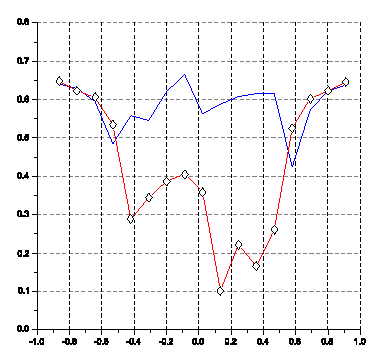
\includegraphics{figure1}
\caption{Example of figure inclusion.}
\label{penG}
\end{figure}

Sample of cross-reference to figure.
Figure~\ref{penG} shows that is not easy to get something on paper.

\section{Headings}

\subsection{Subsection}
Carr-Goldstein based their model on balancing methods and
biochemical know\-ledge. The original model (1980) contained an equation for the
oxygen dynamics which has been omitted in a second paper
(1981). This simplified model shall be discussed here.

\subsubsection{Subsubsection}
Carr-Goldstein
based their model on balancing methods and
biochemical know\-ledge. The original model (1980) contained an equation for the
oxygen dynamics which has been omitted in a second paper
(1981). This simplified model shall be discussed here.

\section{Equations and the like}

Two equations:
\begin{equation}
    C_{s}  =  K_{M} \frac{\mu/\mu_{x}}{1-\mu/\mu_{x}} \label{ccs}
\end{equation}

and

\begin{equation}
    G = \frac{P_{\rm opt} - P_{\rm ref}}{P_{\rm ref}} \mbox{\ }100 \mbox{\ }(\%)
\end{equation}

Two equation arrays:

\begin{eqnarray}
  \frac{dS}{dt} & = & - \sigma X + s_{F} F\\
  \frac{dX}{dt} & = &   \mu    X\\
  \frac{dP}{dt} & = &   \pi    X - k_{h} P\\
  \frac{dV}{dt} & = &   F
\end{eqnarray}

and,

\begin{eqnarray}
 \mu_{\rm substr} & = & \mu_{x} \frac{C_{s}}{K_{x}C_{x}+C_{s}}  \\
 \mu              & = & \mu_{\rm substr} - Y_{x/s}(1-H(C_{s}))(m_{s}+\pi /Y_{p/s}) \\
 \sigma           & = & \mu_{\rm substr}/Y_{x/s}+ H(C_{s}) (m_{s}+ \pi /Y_{p/s})
\end{eqnarray}

\appendix

\section{Appendix section}\label{app}

We consider a sequence of queueing systems
indexed by $n$.  It is assumed that each system
is composed of $J$ stations, indexed by $1$
through $J$, and $K$ customer classes, indexed
by $1$ through $K$.  Each customer class
has a fixed route through the network of
stations.  Customers in class
$k$, $k=1,\ldots,K$, arrive to the
system according to a
renewal process, independently of the arrivals
of the other customer classes.  These customers
move through the network, never visiting a station
more than once, until they eventually exit
the system.

\subsection{Appendix subsection}

However, different customer classes may visit
stations in different orders; the system
is not necessarily ``feed-forward.''
We define the {\em path of class $k$ customers} in
as the sequence of servers
they encounter along their way through the network
and denote it by
\begin{equation}
\mathcal{P}=\bigl(j_{k,1},j_{k,2},\dots,j_{k,m(k)}\bigr). \label{path}
\end{equation}

Sample of cross-reference to the formula \ref{path} in Appendix \ref{app}.

\begin{acks}[Acknowledgments]
And this is an acknowledgements section with a heading that was produced by the
$\backslash$section* command. Thank you all for helping me writing this
\LaTeX\ sample file.
\end{acks}

%%%%%%%%%%%%%%%%%%%%%%%%%%%%%%%%%%%%%%%%%%%%%%
%% Supplementary Material, if any, should   %%
%% be provided in {supplement} environment  %%
%% with title and short description.        %%
%%%%%%%%%%%%%%%%%%%%%%%%%%%%%%%%%%%%%%%%%%%%%%
\begin{supplement}
\stitle{Title of Supplement A}
\sdescription{Short description of Supplement A.}
\end{supplement}
\begin{supplement}
\stitle{Title of Supplement B}
\sdescription{Short description of Supplement B.}
\end{supplement}

\bibliographystyle{imsart-nameyear}
\bibliography{/Users/ekatsevi/.references/crtpower}

\end{document}
